\section{The Intel 486}

\begin{wrapfigure}[5]{r}{0.25\textwidth}
\centering

\includegraphics[width=.25\textwidth]{drawings/intel_logo.pdf}
\end{wrapfigure}

Announced in 1989, the i486-25Mhz was a performance evolution which addressed all bottleneck of the 386 and shipped with an integrating FPU\footnote{Floating Point Unit} named i487. Like for its predecessor (the i386 running Wolfenstein 3D), Intel offered two flavors, an SX version and a DX version (more powerful). This choice was only enabled due to manufacturing problems where some 486 chips came out with malfunctioning FPUs units. Instead of throwing these away, Intel sold them at a discounted price.\\
\par
 On \cw{alt.games.doom} BBS\footnote{Bulletin Board System} one endless thread in particular debated on what to get to play \doom. Should customer go for an SX, should they go for a DX which was supposed to be "faster"\footnote{\cw{alt.games.doom}: Does a 486DX run Doom faster than an SX?}. Comparing simple instruction speed for \cw{integer} and \cw{float} gives us the answer.\\
 \par

\newcolumntype{L}[1]{>{\hsize=#1\hsize\raggedright\arraybackslash}X}%
\newcolumntype{R}[1]{>{\hsize=#1\hsize\raggedleft\arraybackslash}X}%
 \begin{figure}[H]
\centering  
\begin{tabularx}{\textwidth}{ L{0.3} L{0.3} L{0.4}}
  \toprule
  \textbf{Operation} &  \textbf{i486 (ALU)} & \textbf{i487 (FPU)} \\
  \toprule 
   
   \cw{ADD} & 1 & 8-20\\
   \cw{DIV} & 43 & 73\\
   \cw{MUL} & 12-42 & 29-52\\
   \toprule
\end{tabularx}
\caption{Comparaison ALU vs FPU operations.}
\end{figure}
\bigskip
      \par

Even though the Floating Point Unit performance was drastically improved compared to the previous generation (i387), it was still a far cry of what the ALU could deliver with performances up to 20x slower. As a result, video games of the 90s did not have the luxury to use floating point arithmetics. To play \doom, a 486-SX or a 486-DX were exactly the same thing.\\
\par




If in retrospect the 486 is an unquestionable powerhouse (both in terms of performances and sales\footnote{It was still manufactured as late as 2015 for routers}), it was far from a guaranteed success when it was released. Priced at \$950\footnote{\$950 is \$1,920 in 2017, adjusted to inflation.} for the DX 
and \$258\footnote{InfoWorld Apr 29, 1991.}\footnote{\$258 in 1991 is \$469.20 in 2017, adjusted to inflation.} for the SX, the beast left a dent on a wallet. 
On top of its price, the i486 had to face internal competition from an other CPU also manufactured by Intel around the same time, the i860. Relying on an heavily pipelined superscaler architecture crushing VLIWs\footnote{Very long instruction word.}. It three units, X, Y ,and Z allowed parallel processing which rendered it incompatible with the i386 instruction set hard the potential to easily outperform a 486. Where most CPU tried to hide complexity from compiler, the i860 allowed direct access to its parallel pipeline\footnote{https://en.wikipedia.org/wiki/NEAT\_chipset}.\\
\par
\fq{Cray on a Chip\\
\par
The Intel 80860 was an impressive chip, able at top speed to perform close to 66 MFLOPS at 33 MHz in real applications, compared to a more typical 5 or 10 MFLOPS for other CPUs of the time. Much of this was marketing hype, and it never become popular, lagging behind most newer CPUs and Digital Signal Processors in performance.
The 860 has several modes, from regular scaler mode to a superscalar mode that executes two instructions per cycle and a user visible pipeline mode (instructions using the result register of a multi-cycle op would take the current value instead of stalling and waiting for the result). It can use the 8K data cache in a limited way as a small vector register (like those in supercomputers). The unusual cache uses virtual addresses, instead of physical, so the cache has to be flushed any time the page tables changes, even if the data is unchanged. Instruction and data busses are separate, with 4 G of memory, using segments. It also includes a Memory Management Unit for virtual storage.\\
\par
The 860 has thirty two 32 bit registers and thirty two 32 bit (or sixteen 64 bit) floating point registers. It was one of the first microprocessors to contains not only an FPU as well as an integer ALU, and also included a 3-D graphics unit (attached to the FPU) that supports lines drawing, Gouraud shading, Z-buffering for hidden line removal, and operations in conjunction with the FPU. It was also the first able to do an integer operation, and a (unique at the time) multiply and add floating point instruction, for the equivalent of three instructions, at the same time.\\
\par
However actually getting the chip at top speed usually requires using assembly language - using standard compilers gives it a speed closer to other processors. Because of this, it was used as a coprocessor, either for graphics, or floating point acceleration, like add in parallel units for workstations. Another problem with using the Intel 860 as a general purpose CPU is the difficulty handling interrupts. It is extensively pipelined, having as many as four pipes operating at once, and when an interrupt occurs, the pipes can spill and lose data unless complex code is used to clean up. Delays range from 62 cycles (best case) to 50 microseconds (almost 2000 cycles).}{John Bayko, University of Regina}
\par

\fq{

\begin{wrapfigure}[11]{r}{0.55\textwidth}
\centering
\scaledimage{0.55}{i860.png}
\end{wrapfigure}

...We now had two very powerful chips that we were introducing at just about the same time: the 486, largely based on CISC technology and compatible with all the pc software, and the i860, based on RISC technology, which was very fast but compatible with nothing. we didn't know what to do. so we introduced both, figuring we'd let the marketplace decide. however, things were not that simple. supporting a microprocessor architecture with all the necessary computer-related products --- software, sales, and technical support --- takes enormous resources. even a company like Intel had to strain to do an adequate job with just one architecture. and now we had two different and competing efforts, each demanding more and more internal resources. development projects have a tendency to want to grow like the proverbial mustard seed. the fight for resources and for marketing attention (for example, when meeting with the customer, which processor should we highlight) led to internal debates that were fierce enough to tear apart our microprocessor organization. meanwhile, our equivocation caused our customers to wonder what Intel really stood for, the 486 or i860?}{Andy Grove, "Only the paranoid survive".}
\bigskip
\par
In practice however the i860 never stood a chance. Impaired by its audacious yet incompatible instruction set, only its superior design could have saved sales. With compiler technology still struggling to generate fast C properly, nothing was even remotely close to generate instructions able to exploit its super scalar capability. If only Intel had been willing to build the compilers it desperately needed the i860 history could have been different.\\
\par
\trivia{Amusingly, the i860 would still play a part in Doom's development since it was used on NextDimension boards.}
\par

\par
\subsection{Performance improvements}
Charting the 486 performances against the previous 386 showed a tremendous improvement. The first obvious reasons was the raw increase of frequency. Where Intel offered up to 40 Mhz on a 386, the smaller process of the 486 allowed up to 50 Mhz, giving it an obvious advantage. But looking close at the chart, one will notice that even at equal frequency, a 486 offered more than twice the processing power of a 386.\\

\par
\begin{figure}[H]
\centering
  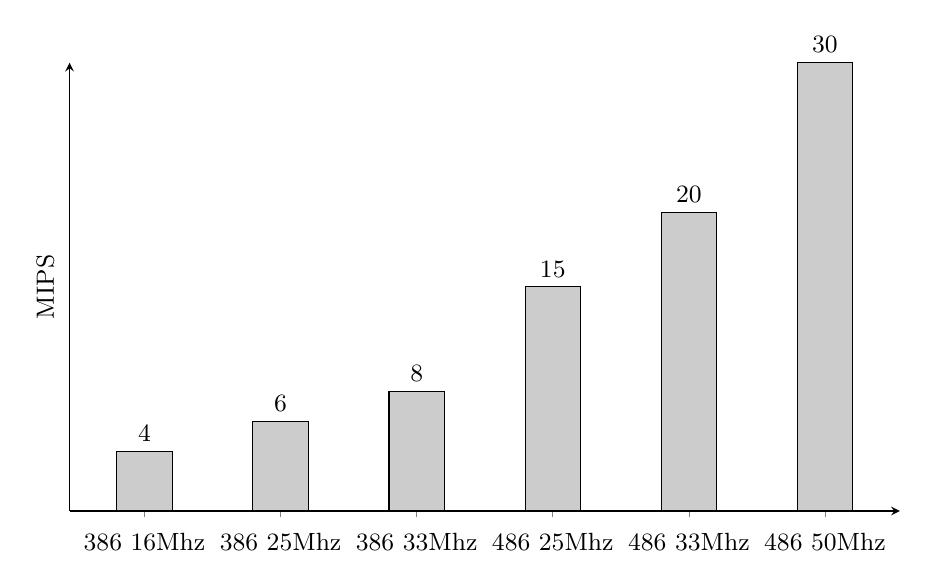
\begin{tikzpicture}[font=\small]
    \begin{axis}[
      width=1.0\textwidth,
      height=0.6\textwidth,
      ybar,
      bar width=20pt,
      ylabel={MIPS},
      ymin=0,
      ytick=\empty,
      xtick=data,
      axis x line=bottom,
      axis y line=left,
      enlarge x limits=0.11,
      symbolic x coords={386 16Mhz,386 25Mhz,386 33Mhz,486 25Mhz,486 33Mhz,486 50Mhz},
      xticklabel style={anchor=base,yshift=-\baselineskip},
      nodes near coords={\pgfmathprintnumber\pgfplotspointmeta}
    ]
      \addplot[fill=black!20,draw=black] coordinates {
        (386 16Mhz,4)
        (386 25Mhz,6)
        (386 33Mhz,8)
        (486 25Mhz,15)
        (486 33Mhz,20)
        (486 50Mhz,30)
      };
    \end{axis}
   
   \end{tikzpicture}
   \caption{Comparison\protect\footnotemark of CPUs with MIPS \protect\footnotemark.}
 \end{figure}
\footnotetext{Source: "Roy Longbottom's PC Benchmark Collection: http://www.roylongbottom.org.uk/mips.htm".}

Intel had identified all bottlenecks in the 486 and fixed them. The name of the game was to avoid ALU starvation in terms of both instructions and operands.\\
\par
\cscaledimage{0.6}{i486DX.png}{The Intel 486 packing 1.2 millions transistors.}
\par













According to Intel 80386 programmer's reference manual from 1986, their processor was a three stage pipeline which was ideally always full and busy.\\
\par
\begin{figure}[H]
\centering
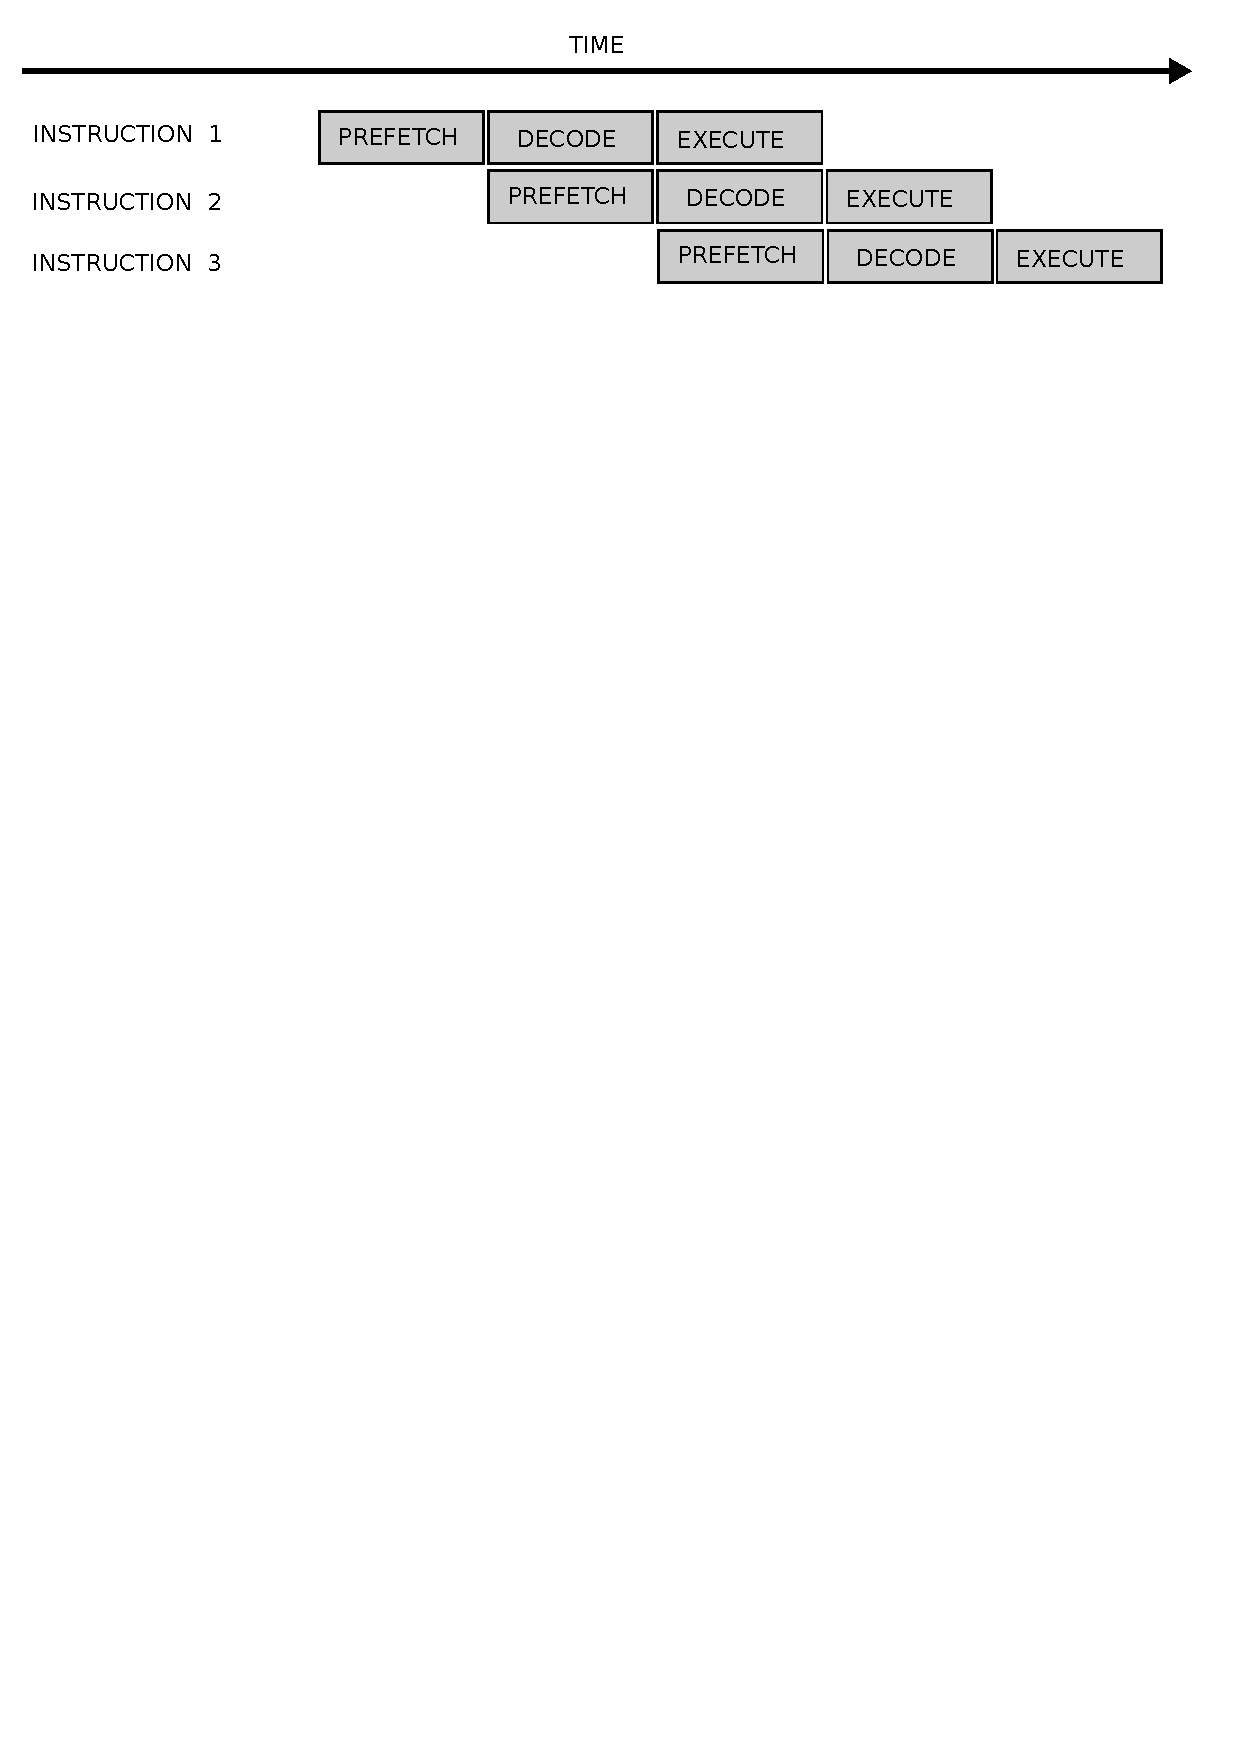
\includegraphics[width=\textwidth]{drawings/386_instruction_pipeline.pdf}
\caption{386 pipeline in Intel documentation.}
\end{figure}
\bigskip
\par
In practice however, even if the Prefetch Unit and the Execution Unit were properly fed, the Decode unit always took a minimum of two cycles to decode an instruction\footnote{The author speculates this high decode cost was the result of Intel's choice to use CISC instead of RISC.}. Since the maximum throughput of a pipeline cannot exceed the speed of its slowest stage, the Intel 386 could process at its most one instructions every two cycles.\\
\par

\begin{figure}[H]
\centering
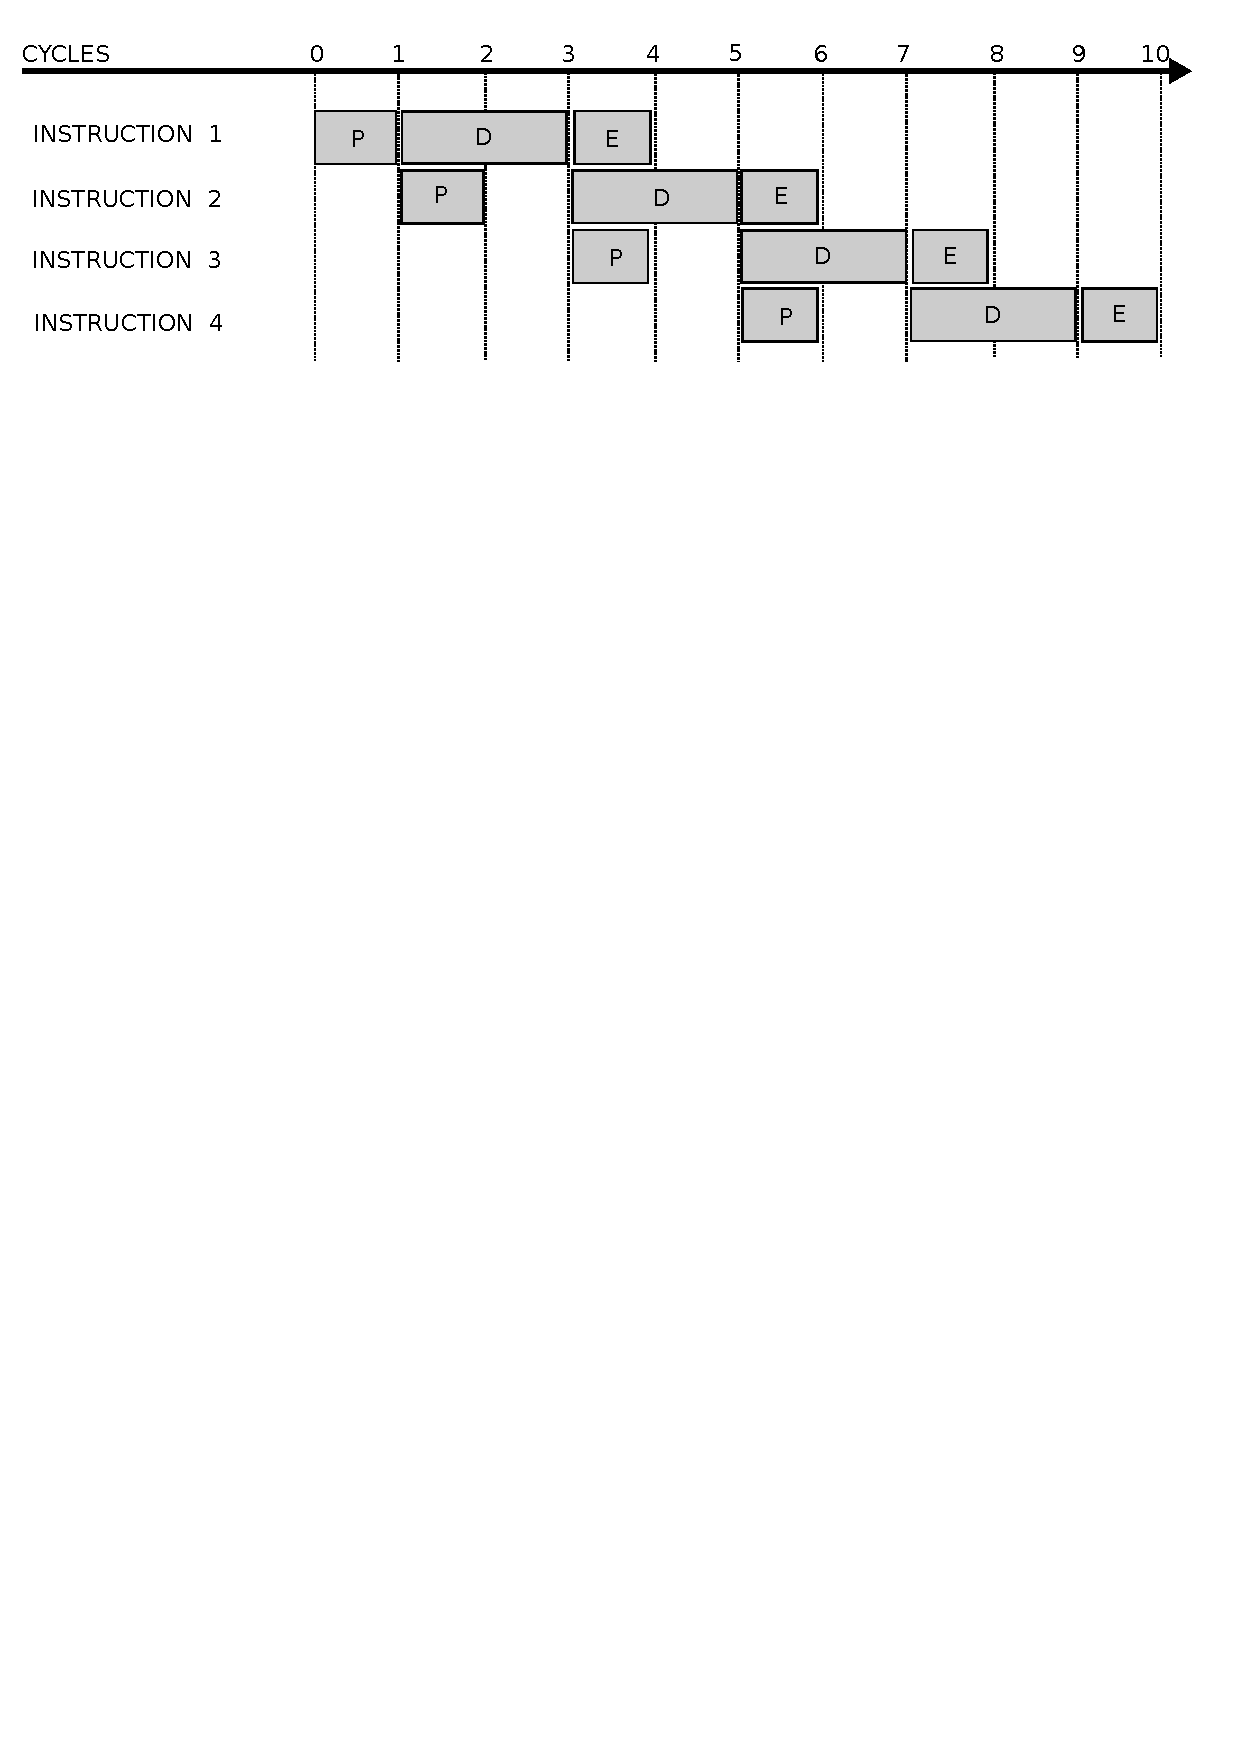
\includegraphics[width=\textwidth]{drawings/actual_386_instruction_pipeline.pdf}
\caption{386 pipeline: Two cycles per instruction.}
\end{figure}
\bigskip
\par
To solve this problem, Intel simply decided to break the three stage pipeline into four (plus an other stage explained later). With all stages performing at 1 CPI, the total throughput of the 486 was doubled.\\
\begin{figure}[H]
\centering
\includegraphics[width=\textwidth]{drawings/actual_486_instruction_pipeline.pdf}
\caption{486 pipeline: One cycle per instruction.}
\end{figure}
\par





\subsection{Caching }
To fix the pipeline and make each stage even was important but the real important problem to avoid at all cost were stales due to either instruction or operand starvation. four-way set-associative write through.\\

\subsection{DRAM vs SRAM}
\subsection{Cache L2}
Bla
\subsection{Precaching (cachelines) Netburst}
Bla


\begin{figure}[H]
\centering
\scaledimage{0.9}{486_blueprint.png}
\end{figure}
\par
\begin{figure}[H]
\centering
\scaledimage{0.9}{486_layout.png}
\end{figure}








\section{Overdrive, 486 DX2 66Mhz}

\begin{figure}[H]
\centering

\includegraphics[width=\textwidth]{drawings/486dx2_notm.pdf}
\end{figure}
\par


\begin{figure}[H]
\centering
  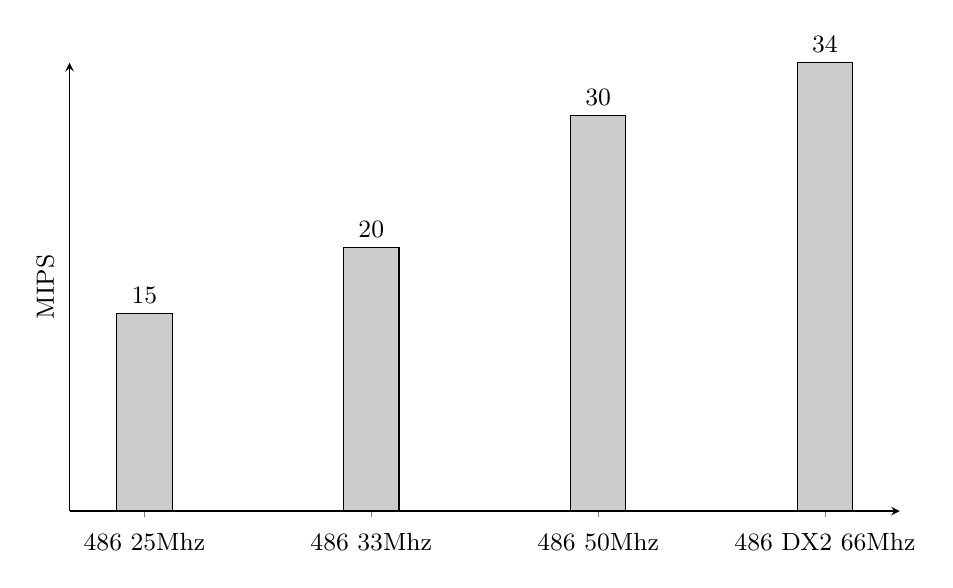
\begin{tikzpicture}[font=\small]
    \begin{axis}[
      width=1.0\textwidth,
      height=0.6\textwidth,
      ybar,
      bar width=20pt,
      ylabel={MIPS},
      ymin=0,
      ytick=\empty,
      xtick=data,
      axis x line=bottom,
      axis y line=left,
      enlarge x limits=0.11,
      symbolic x coords={486 25Mhz,486 33Mhz,486 50Mhz,486 DX2 66Mhz},
      xticklabel style={anchor=base,yshift=-\baselineskip},
      nodes near coords={\pgfmathprintnumber\pgfplotspointmeta}
    ]
      \addplot[fill=black!20,draw=black] coordinates {
        (486 25Mhz,15)
        (486 33Mhz,20)
        (486 50Mhz,30)
        (486 DX2 66Mhz,34)
      };
    \end{axis}
   
   \end{tikzpicture}
   \caption{Comparison\protect\footnotemark of CPUs with MIPS \protect\footnotemark.}
 \end{figure}
\footnotetext{Source: "Roy Longbottom's PC Benchmark Collection: http://www.roylongbottom.org.uk/mips.htm".}

Zero-wait state.\\
DRAM vs SRAM\\
Cache hit percentage from ISA book.\\
four-way set-associative write back.\\


\subsection{Performance \& Price}
By may 1992, the Intel 386 was being replaced by a new version, the 486. The increase in operatin frequency was substancial for the high end model running at 50Mhz but most 486 ran at the same speed at the 386: 25Mhz and 33Mhz. The revolutionary design of the CPU.\\
\par
TODO: How to program it? Use the cache luke and avoid branching. Re-read michael abrash guide on 486.
\subsection{Floating Point Unit}
The i386 was able to talk to an i387 located on the motherboard. Requests and responses had to transition on the bus and incurred four CPU cycles of overhead. For the i486, Intel decided to integrate the i487 FPU in the same die and improved performance by a factor 2.\\
\par
TODO: Drawing
\par

TODO: Verify with 387/487 description

\subsection{Fixed Point arithmetic}

\par
\begin{figure}[H]
\centering
\begin{tabularx}{\textwidth}{ X  X X  X  X}
  \toprule
  \textbf{CPU} & \textbf{FADD} & \textbf{FMUL} & \textbf{FDIV} &\textbf{FXCH} \\ \bottomrule
Intel 387 & 23-34 & 29-57   & 88-91 & 18 \\
Intel 487 & 8-20  & 16   & 73 & 4 \\ \bottomrule
\end{tabularx}
\caption{FPU performance: 387 vs 487.}
\label{perf_summary}
\end{figure}